% !TEX encoding = UTF-8
% !TEX program = pdflatex
% !TEX root = InformationRetrieval.tex
% !TEX spellcheck = it-IT

% 18 Novembre 2016
%\chapter{Valutazione dei sistemi di reperimento}
%\section Il paradigma Cranfield

\section{Recall}

Il richiamo misura quanti documenti rilevanti sono stati recuperati, rispetto la totalità dei documenti rilevanti presenti all'interno del pool. Anche in questo caso si tratta di un valore compreso tra 0 e 1, dove 1 indica la run perfetta.

\begin{figure}[htbp]
	\centering
	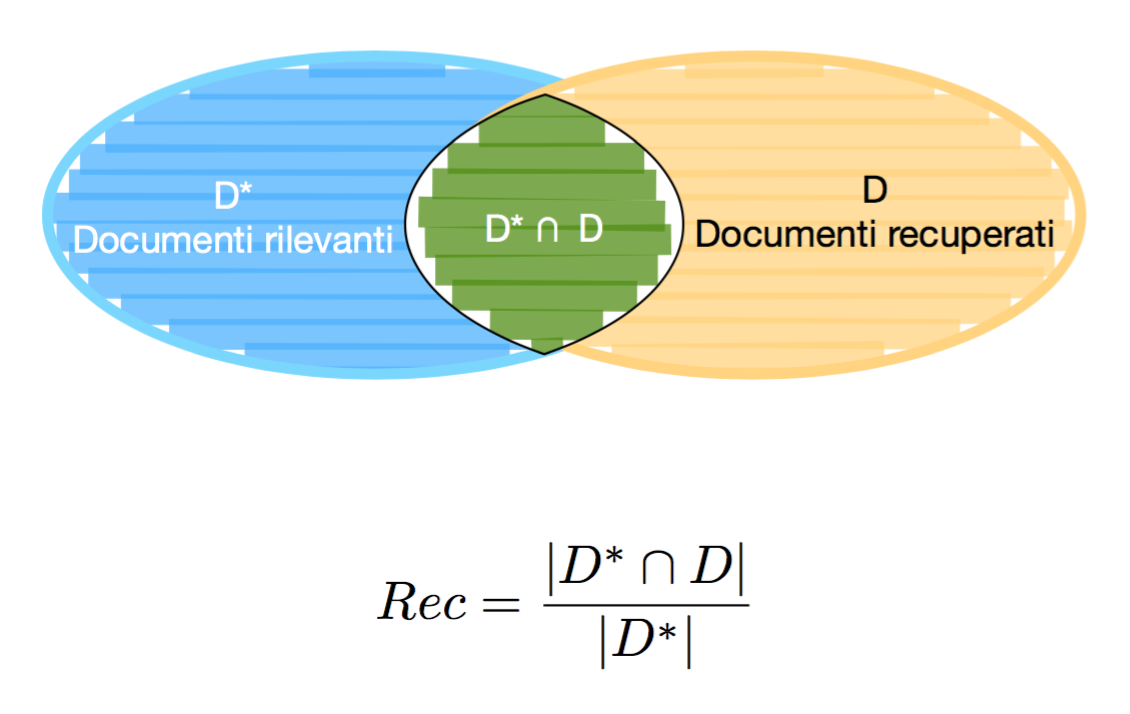
\includegraphics[width=0.6\textwidth]{images/l15-fig-1.png}
\end{figure}

Il valore $|D^*|$ è anche chiamato \textbf{recall base} per un determinato topic e come già detto è valore fisso che dipende dal numero di documenti rilevanti presenti nel pool o ground truth.

Più formalmente, sia $D$ un insieme finito di documenti, $T$ un insieme finito di topic, $GT$ la ground truth defin ita su $D$ e $T$ e rel un insieme totalmente ordinato di giudizi di rilevanza. La \textbf{recall base} è definita come:

\begin{align*}
	RB : T &\to \mathbb{N} \\
		t &\to RB_t = \Big| \big\{ d \in D | GT(t,d) \succ \min(REL) \big\} \Big|
\end{align*}

\begin{figure}[htbp]
	\centering
	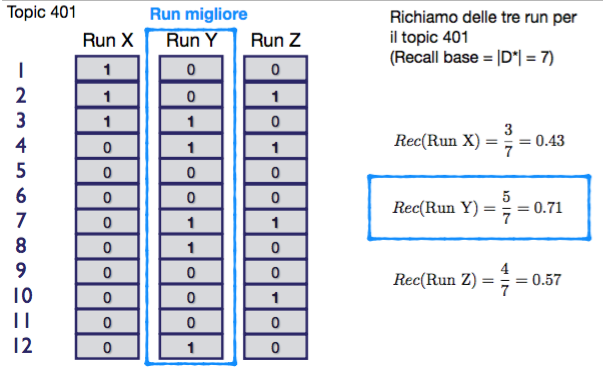
\includegraphics[width=0.7\textwidth]{images/l15-fig-2.png}
	\caption{Esempio di calcolo della recall.}
\end{figure}

\section{E-Measure e F-measure}

\`E utile avere un numero unico per esprimere la qualità della run e che riesca a combinare la precisione e il richiamo

\begin{figure}[htbp]
	\centering
	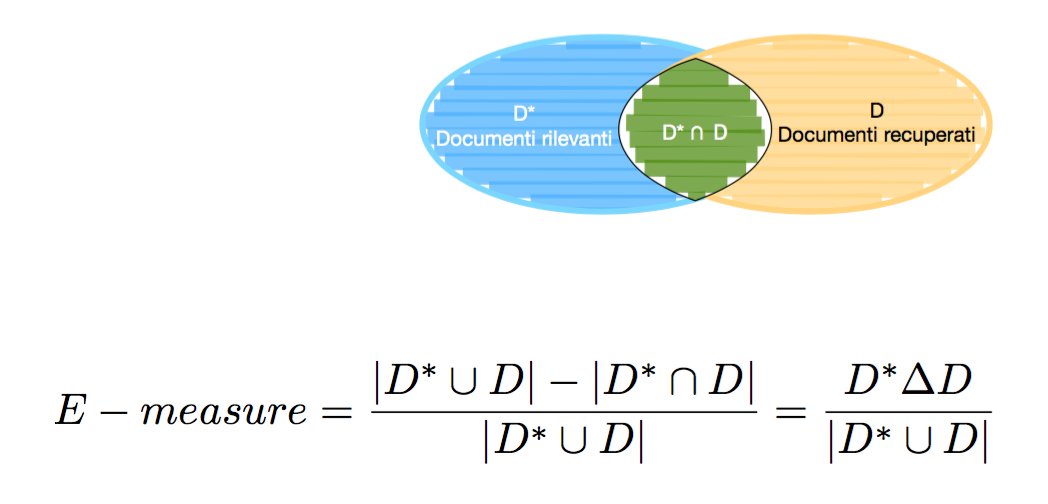
\includegraphics[width=0.7\textwidth]{images/l15-fig-3.png}
\end{figure}

Se l'intersezione è vuota, ottengo un e-measure è 1, che è il caso di retrieval pessimo.
Se invece l'e-meausre è 1, i due insiemi coincidono e quindi il retrieval è perfetto.

Siccome questa misura è contro-intuitiva si è scelto di utilizzare

$$
F-measure = 1 - E\text{-}measure
$$

Tuttavia, anche questa misura, come precision e recall, non è una misura ranked, perché non viene preso in considerazione l'ordine.


\section{Precisione con cut-off}

Per alcuni task di ricerca è importante tenere in considerazione l'ordine dei risultati e quindi è utile avere delle misure che tengano conto anche di questo.

L'idea quindi è quella di calcolare la precisione solamente sui primi $k$ elementi recuperati. Questa nuova misura prende il nome di $perc@k$.

Un caso particolare è quello di $p[RB_t]$ che è la precision con cut-off dato dalla dimensione della recall base per un dato topic.

\section{Curva Richiamo-Precisione}

Questa curva calcola la precisione in funzione di $x$ punti di richiamo, in modo da poter disegnare una curva con i punti di richiamo sull'asse delle ascisse e la precisione sulle ordinate.

\begin{figure}[htbp]
	\centering
	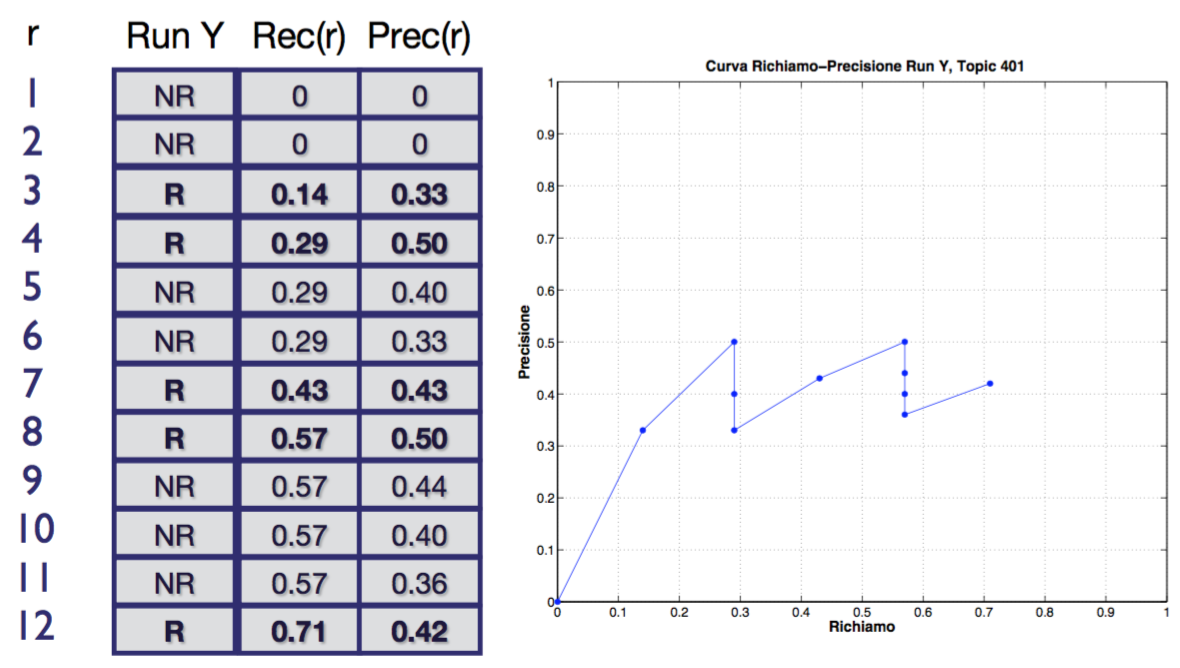
\includegraphics[width=0.6\textwidth]{images/l15-fig-4.png}
	\caption{Esempio della curva richiamo-precisione.}
\end{figure}

Ovvero per ogni livello di rango vengono calcolate la precisione e il richiamo con cut-off a quel livello.

Questa curva però ha un sacco di problemi, perché intanto non è una funzione, inoltre non è possibile utilizzarla per comparare due run distinte. C'è poi anche da tenere in considerazione che uno stesso sistema può produrre run diverse.

Una variante è la curva \textbf{interpolata}: una curva simile che viene ottenuta considerando 11 punti fissi di richiamo (\textbf{11-point recall-precision}):

$$
rp \in \{ 0, 0.1, 0.2, \ldots 1 \}
$$

e viene calcolata come 

$$
IP_{rp} = \max_{1 \leq r \leq N | Rec(r) \geq rp} Prec(r)
$$

ovvero, ad ognuno dei punti dell'insieme $rp$ viene associato il più alto valore di precisione ottenuto sui primi $r$ valori della run che hanno un richiamo maggiore del punto.

\begin{figure}[htbp]
	\centering
	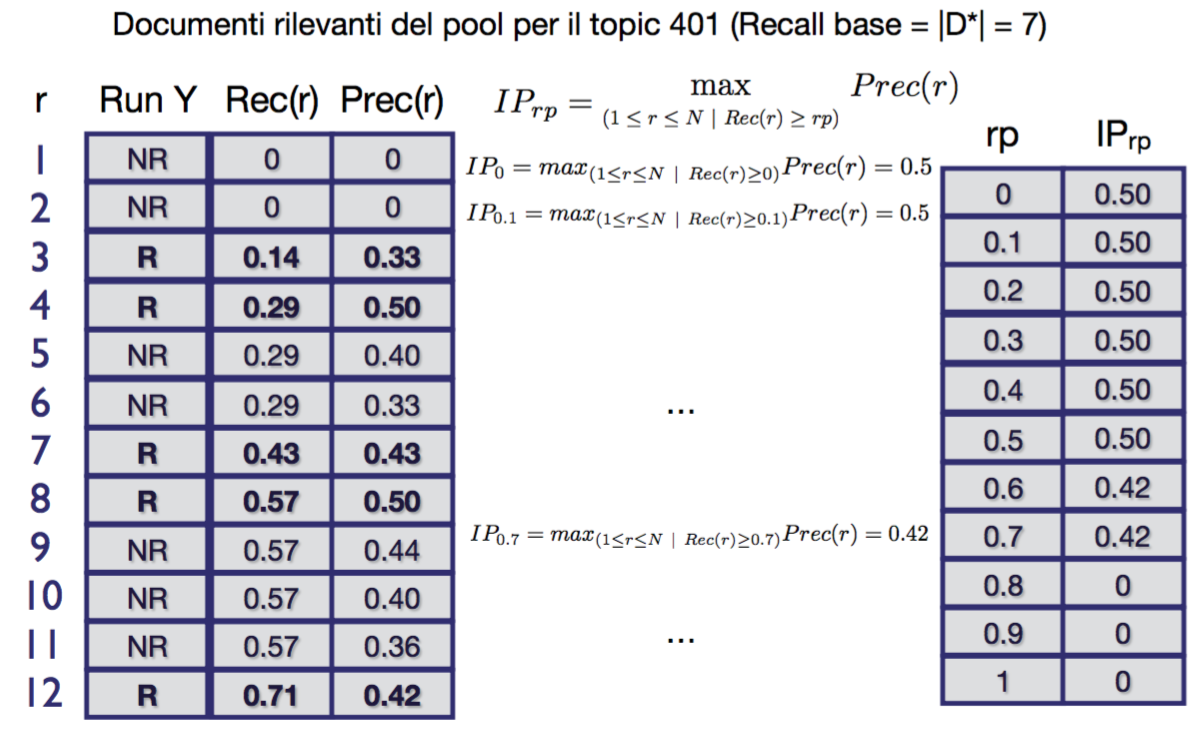
\includegraphics[width=0.6\textwidth]{images/l15-fig-5.png}
	\caption{Esempio di calcolo della curva richiamo-precisione interpolata.}
\end{figure}

\begin{figure}[htbp]
	\centering
	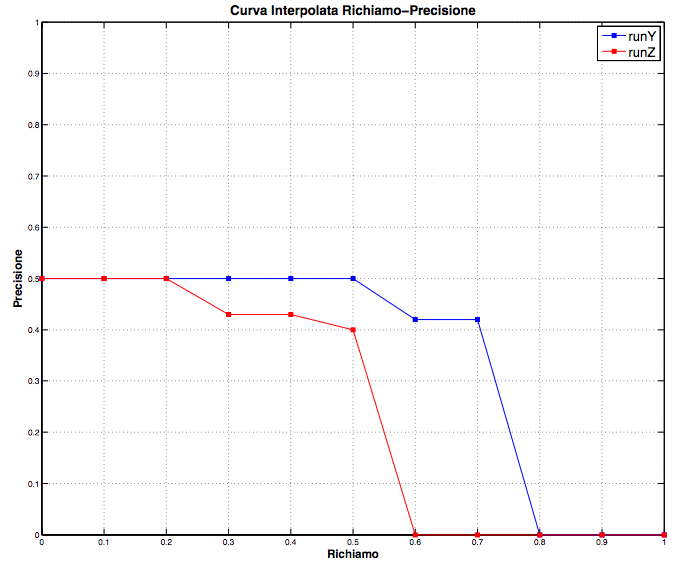
\includegraphics[width=0.4\textwidth]{images/l15-fig-6.png}
	\caption{Esempio di curva richiamo-precisione interpolata.}
\end{figure}


Questa curva va bene per giudicare ad occhio quale delle due curve va meglio, però si può fare di più utilizzando l'11-\textbf{Point Average Precision} che effettua la media di tutti i valori di precisione interpolata calcolati.

$$
\text{11pt-AP} = \frac{\sum_{rp\in\{0,0.1,\ldots 1 \}}IP_{rp}}{11}
$$

C'è però un'effetto indesiderato perché la precisione a valori alti di richiamo ha lo stesso peso di quelli a livelli bassi.

Tipicamente si usa quindi l'\textbf{Average Precision} che è la misura attualmente più utilizzata.

Dato un topic $t \in T$, una recall base $RB_t$, $REL =\{ nr, r \}$ e una run $r_t$ di lunghezza $N$ tale che:

$$
\forall i \in [1, N], \tilde{r}_t = \begin{cases}
0 \quad &\text{se } \hat{r}_t[i] = nr \\
1 \quad &\text{se } \hat{r}_t[i] = r \\
\end{cases}
$$

l'average precision è quindi definita come:

$$
AP = \frac{1}{RB_t}\sum\limits_{k=1}^{N}\tilde{r}_t[k]\frac{\sum\limits_{h=1}^{k} \tilde{r}_t[h]}{k}
$$

Le misure di questo tipo prendo il nome di \textbf{top heavy} perché danno più peso ai documenti rilevanti in posizioni alte del rank.

\begin{figure}[htbp]
	\centering
	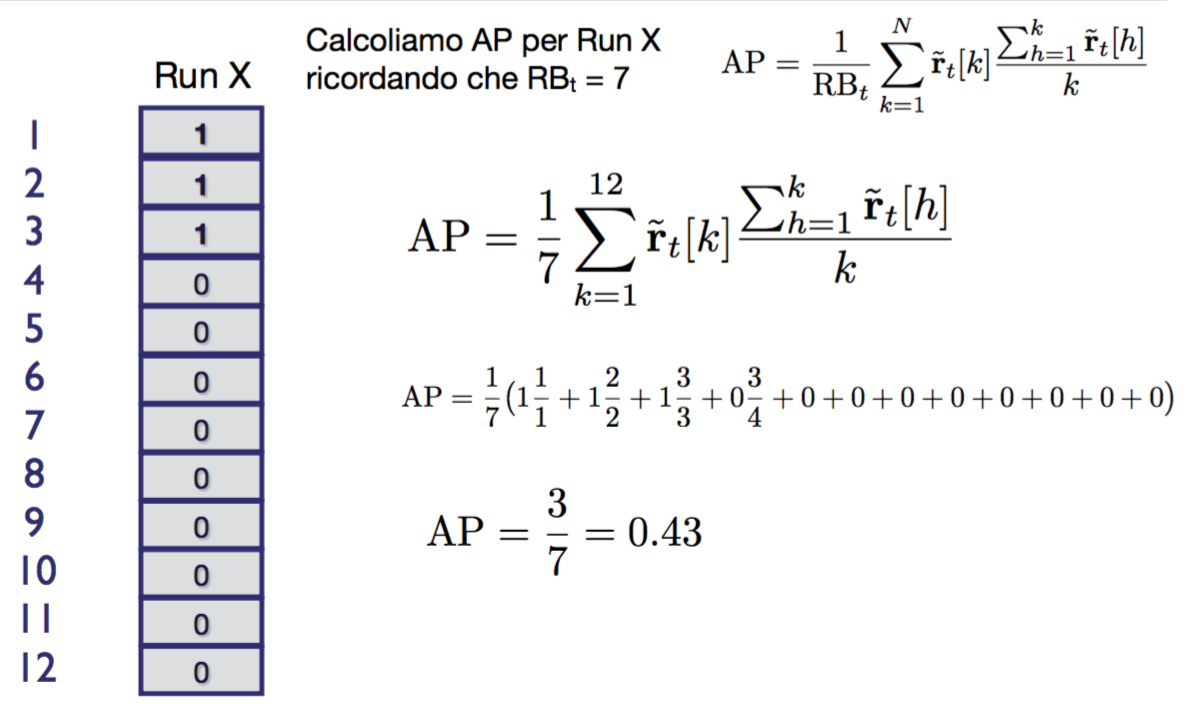
\includegraphics[width=0.7\textwidth]{images/l15-fig-7.png}
	\caption{Esempio di calcolo di Average Precision.}
\end{figure}

\section{Valutazione di un sistema su più topic}

Le misure viste finora valutano la singola run su un topic, ma tipicamente le campagne di valutazione sono fatte su 50 o 100 topic.

L'idea base è quella di fare la media aritmetica delle run sui singoli topic. Si parla quindi di \textbf{Mean Average Precision} (\textbf{MAP}). Detta anche la \textit{media media precisione}.

$$
MAP(R) = \frac{\sum_{t\in T}AP(r_t)}{|T|}
$$

Tipicamente è una brutta idea fare la media di una misura che dipende dalla recall base. Ma nel campo di valutazione dell'IR, AP è una misura che piace e quindi si fa comunque la media. 

Quindi \textbf{MAP} bene, \textbf{R-prec-media} male.
